\documentclass[9pt,a4paper]{report}
\usepackage{mwe}
\usepackage{listings}
\usepackage{amsmath}
\usepackage{graphicx}
\usepackage{subfig}
\usepackage{float}
\usepackage{xcolor}
\usepackage{multirow}
\usepackage{hyperref}
\usepackage{fancyhdr}
\usepackage{sectsty}
\usepackage[dvipsnames]{xcolor}
\usepackage{soul}
\usepackage[compact]{titlesec}
\usepackage{float}
\usepackage[left=0.5cm,right=0.5cm,top=0.5cm,bottom=0.5cm]{geometry}
\graphicspath{{2.1}{2.1/Spice}{2.2}}

\newcommand*{\nchapter}[1]{%
	\chapter*{#1}%
	\addcontentsline{toc}{chapter}{#1}
	\vspace{-14mm}}
\newcommand*{\nsection}[1]{%
	\section*{#1}%
	\addcontentsline{toc}{section}{#1}}
\newcommand*{\nsubsection}[1]{%
	\subsection*{#1}%
	\addcontentsline{toc}{subsection}{#1}}
\newcommand*{\nsubsubsection}[1]{%
	\subsubsection*{#1}%
	\addcontentsline{toc}{subsubsection}{#1}}

\chaptertitlefont{\large}
\sectionfont{\normalsize}
\fontsize{9}{11}\selectfont
\begin{document}
	\begin{titlepage}
		\centering
		\vspace*{1.5in}
		
\includegraphics[width=0.15\textwidth]{W-Logo_Purple_RGB}\par\vspace{1cm}
		{\LARGE \textsc{University of Washington}\par}
		\vspace{1cm}
		{\Large \textsc{BEE331 Lab 2.1}\par}
		\vspace{1.5cm}
		{\huge\bfseries \par}
		\vspace{2cm}
		{\Large\itshape 2301991\hspace{55pt}2130474\par}
		{\Large\itshape Jason Truong\hspace{31pt}Henry Haight\par}
		\vfill
		supervised by\par
		Prof.~Joseph \textsc{Decuir}
		\date{2024\\ January}
		\vfill
		% Bottom of the page
		{\large \today\par}
		\vspace*{1.5in}
	\end{titlepage}
	
		\nchapter{Characterising MOSFET; I-V Curve}
	
	\nsection{Design Objective}
	In this lab, we introduce ourselves to the MOSFET, we characterise its function $V_{DS}$ and $I_D$ curve; related to Triode, Threshold, and Saturation.
	\begingroup
	\renewcommand{\cleardoublepage}{}
	\renewcommand{\clearpage}{}
	\nsection{Circuit Design Outline}
	\endgroup
	With an NMOS (2N7000) Transistor in series from Voltage Input $V_{DD}=12V$ to a resistor ($R_D=100\Omega$), the voltage drop in $V_{DS}=V_D-V_S$, to ground. In the Gate $V_G$ over the capacitor of the MOSFET; in series with a resistor ($R_G=1k\Omega$), being supplied with it's own voltage source; $V_{GG}$.\\\\
	The demonstrated circuits below use a sinusoidal sweep with $V_{DD}$ and $V_{GG}$ respectively to demonstrate the $I_D$ relation over a voltage-change.
	\begin{figure}[hp!]
		\centering
		\caption{\centering 2N7000 NMOS}
		\subfloat[\centering LTSpice + Rudimentary Schematic $I_D$ vs $V_{GS}$ Sweep]{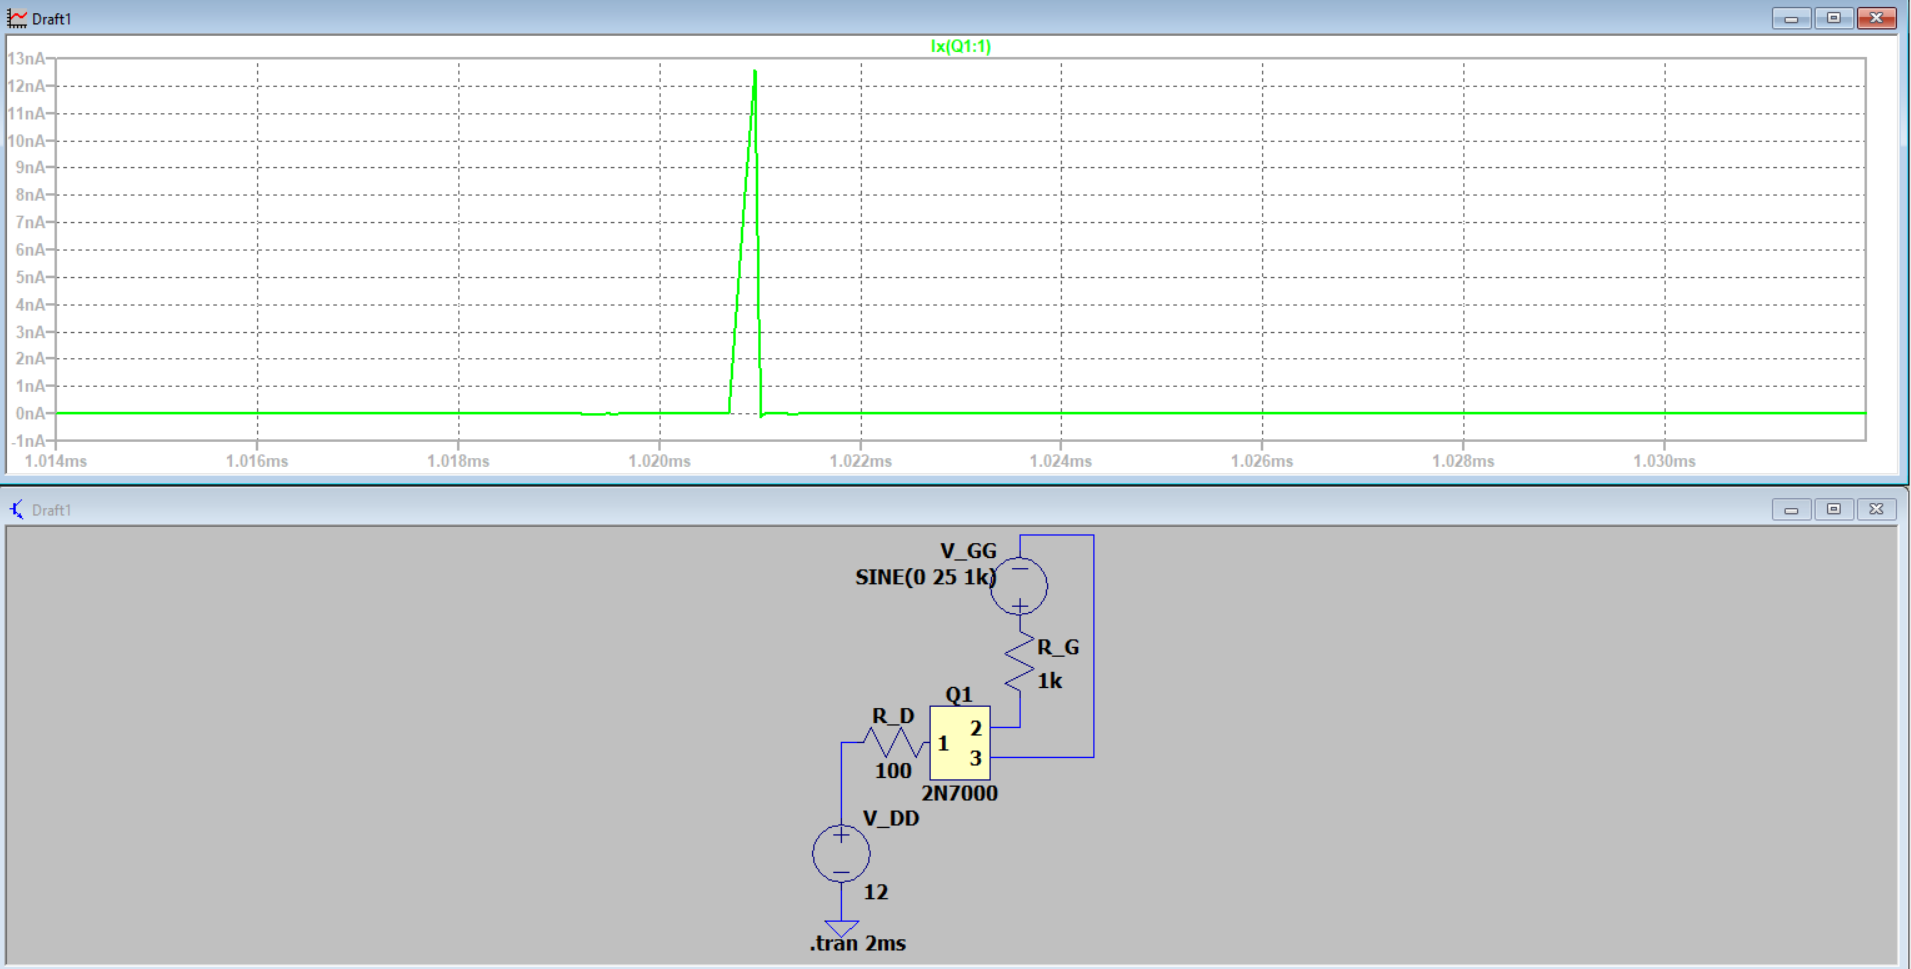
\includegraphics[width=9cm]{Spice Sim Sweep}}\hfil
		\subfloat[\centering LTSpice + Rudimentary Schematic $I_D$ vs $V_{DS}$ Sweep]{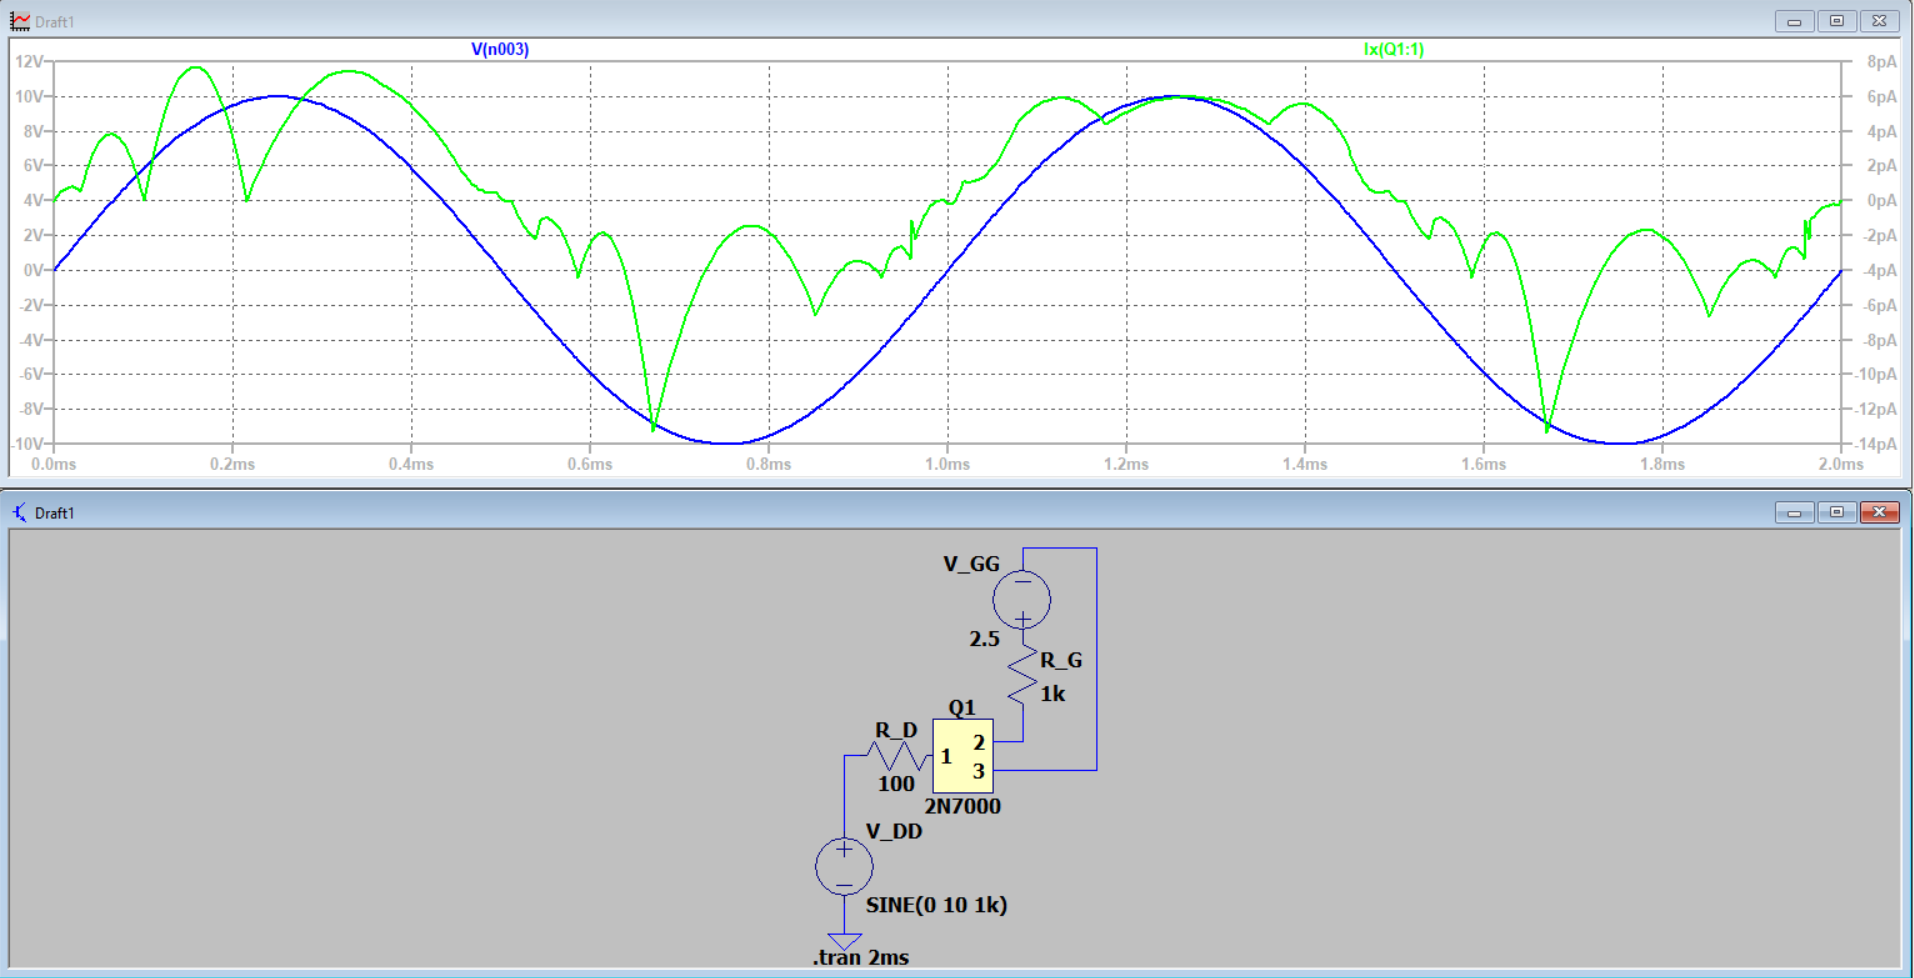
\includegraphics[width=9cm]{ID vs VGS Sweep}}
	\end{figure}
	\begin{figure}[hp!]
		\ContinuedFloat
		\centering
		\subfloat[\centering 2N7000 NMOS Transistor MOSFET Circuit]{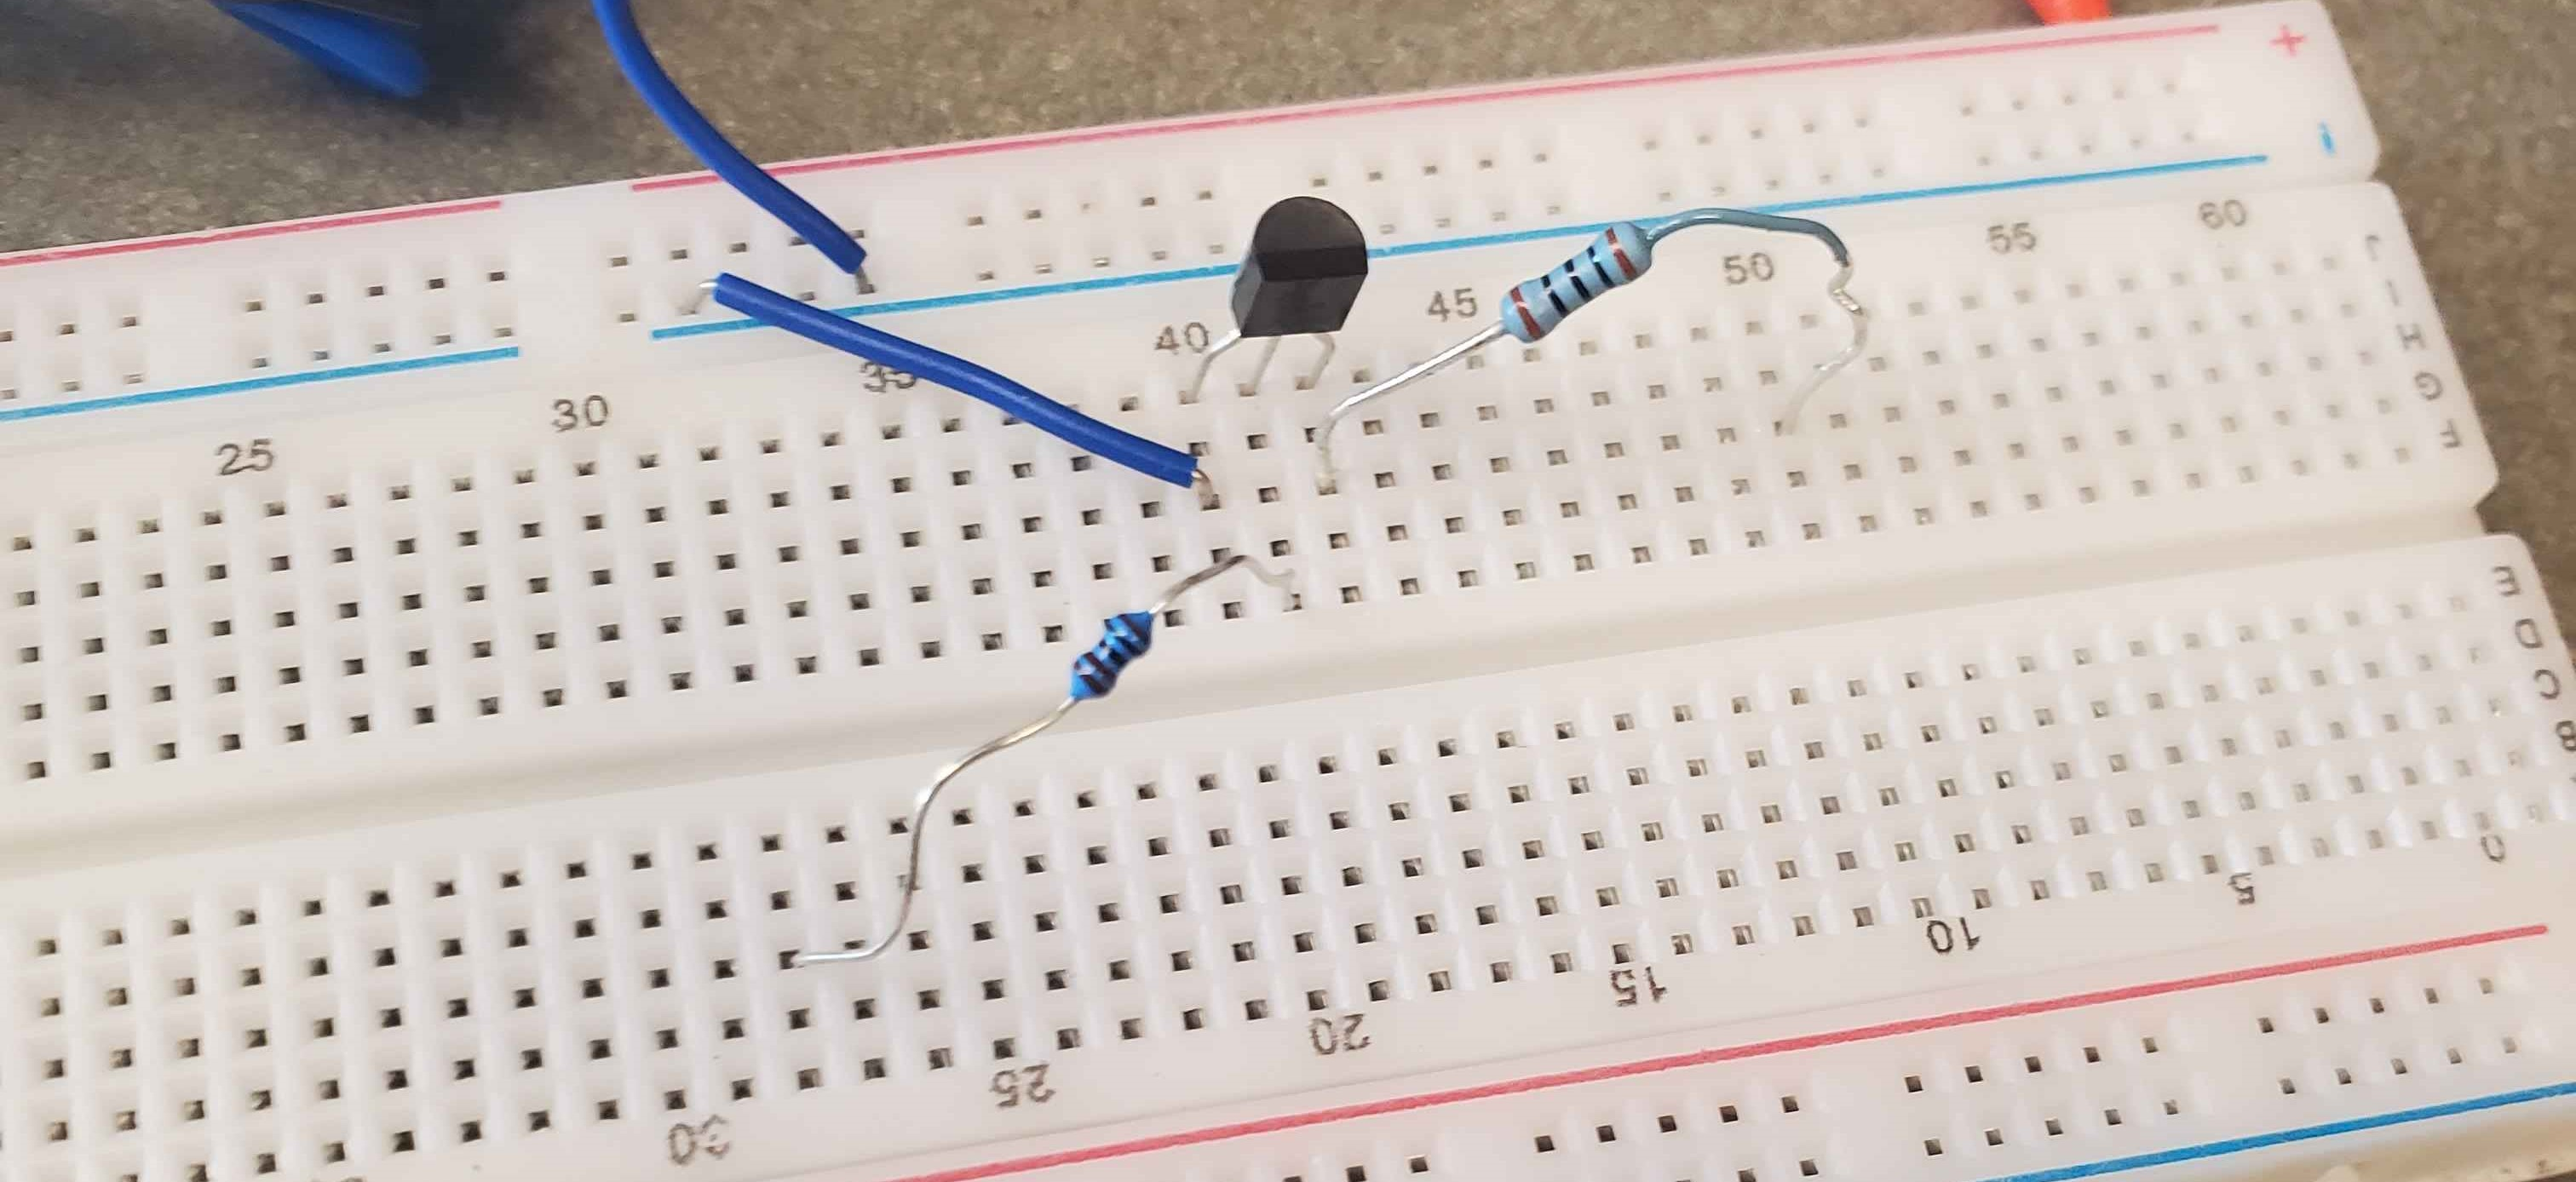
\includegraphics[width=18cm]{2N7000 Transistor Loaded}}
	\end{figure}
	
	\newpage
	\nsection{Descriptions of Measurements \& Calculations}
	\nsubsection{Analysis}
	\begin{itemize}
		\item \textbf{i. Use your plot (or data) to find the value of $V_{GS}$ which just starts to produce a non-zero drain current. This is the threshold voltage $V_t$ of the MOSFET under test.}
		\subitem See below for tables and graphs of [$I_D$ vs $V_{GS}$], and [$I_D$ vs $V_{GS}$].
		\item \textbf{ii. How close are the measured and calculated values of $V_{DS}$ at the boundary of triode and saturation regions of the MOSFET?}
		\subitem \textit{$V_{GS}$ vs $I_D$}: From when the current has a measurable rating ($1.8V$), saturates at a $0.6V$ difference ($2.4V$).
		\subitem \textit{$V_{DS}$ vs $I_D$}: From when the current plateaus at its greatest amount ($1V$ to $1.5V$), saturates at a $.5V$ difference (@$1.5V$). Then proceeds to break the component's specifications by breaching current at around $5V$
		\item \textbf{What model parameters of the MOSFET would you adjust (and how) to match the experimental results?}
		\subitem To simulate the $I_D$ change over a voltage change for [Saturation] and [To $10V$] respectively, we AC-swept over a region.\\
		Aside from the simulation-method, here is the Github link to the .lib model we used to simulate the \href{https://github.com/pepaslabs/LTSpice-parts/blob/master/parts/transistor/mosfet/nchannel/2N7000.nxp.lib}{2N7000 component}.
		\item \textbf{Do the values of $k_n$ obtained from measurements agree with $k_n$ obtained from the model?}
		\subitem Simply, yes; given $k_n=(\frac{I_D*2}{V_{RD}-1.6})^2$
	\end{itemize}
	\begin{figure}[hp!] %140, 
		\centering
		\caption{NMOS Circuits}
		\subfloat[$V_{GS}$ vs $I_D$ Graph]{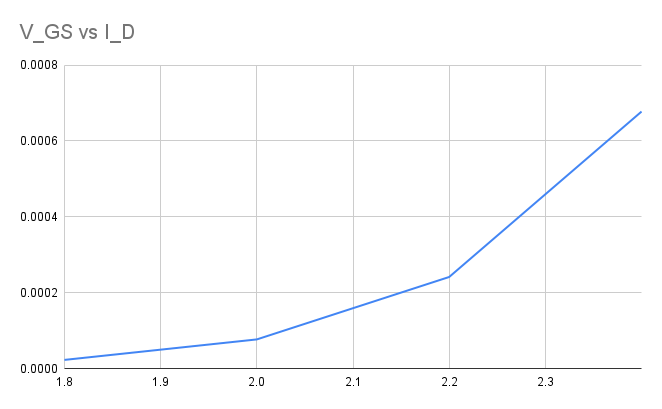
\includegraphics[width=9cm]{V_GS vs I_D Graph}}
		\subfloat[Lab 2 2-2A-I Table]{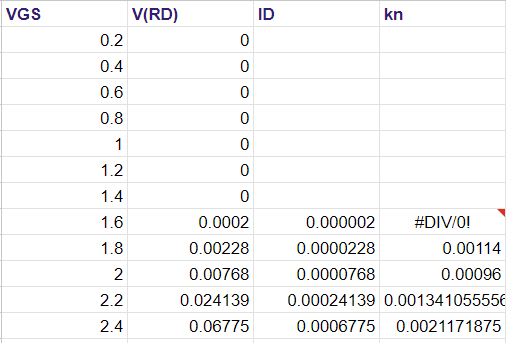
\includegraphics[width=9cm]{Lab 2 2-2A-I Table}}
	\end{figure}
	\begin{figure}[hp!]
		\ContinuedFloat
		\centering
		\subfloat[$I_D$ vs $V_DS$]{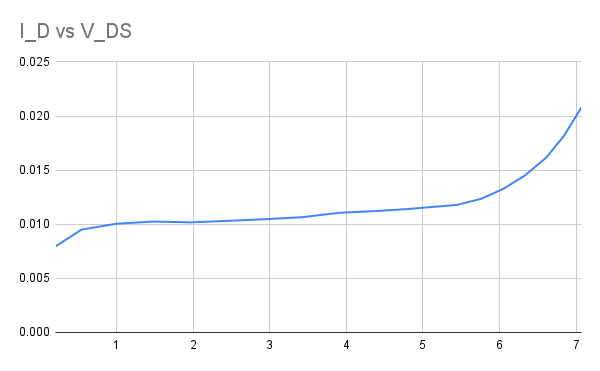
\includegraphics[width=9cm]{I_D vs V_DS}}
		\subfloat[Lab 2 2-2A-I Table]{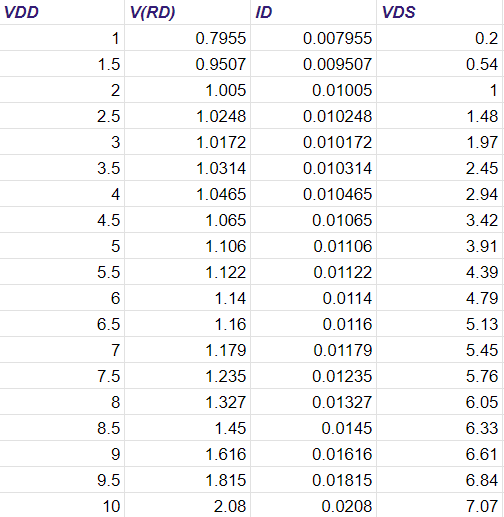
\includegraphics[width=9cm]{Lab 2-2-2A-II Table}}
	\end{figure}
	\begin{figure}[hp!]
		\ContinuedFloat
		\centering
		\subfloat[$I_D$ vs $V_DS$ @$V_{GS}=2.5V$]{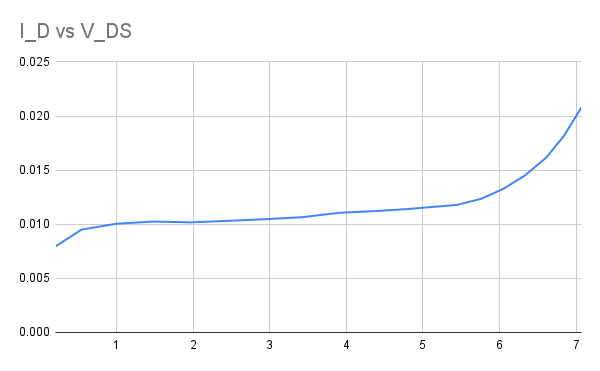
\includegraphics[width=9cm]{I_D vs V_DS}}
		\subfloat[Lab 2 2-2A-I Table @$V_{GS}=2.5V$]{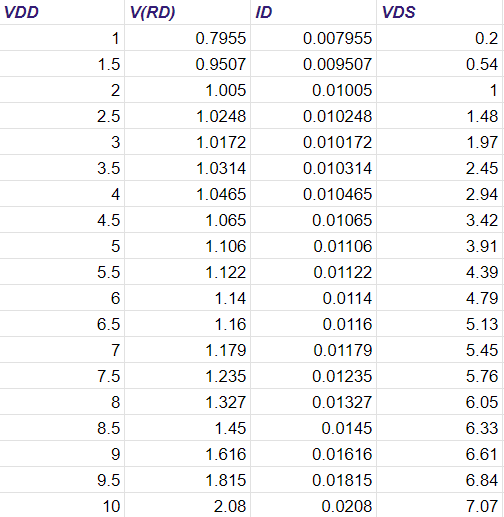
\includegraphics[width=9cm]{Lab 2-2-2A-II Table}}
	\end{figure}
	\begin{figure}[hp!]
		\ContinuedFloat
		\centering
		\subfloat[$I_D$ vs $V_DS$ @$V_{GS}=3V$]{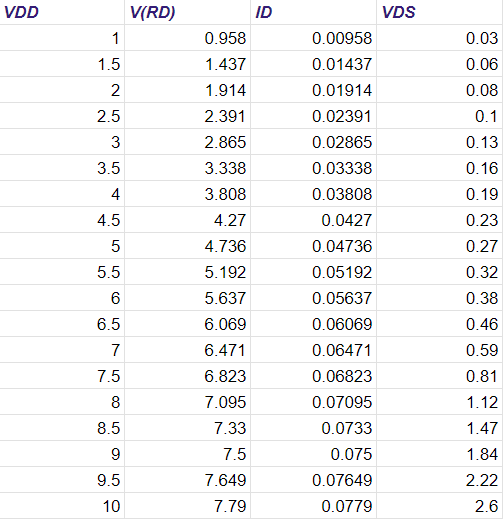
\includegraphics[width=9cm]{Screenshot 2024-07-31 035815}}
		\subfloat[Lab 2 2-2A-I Table @$V_{GS}=3V$]{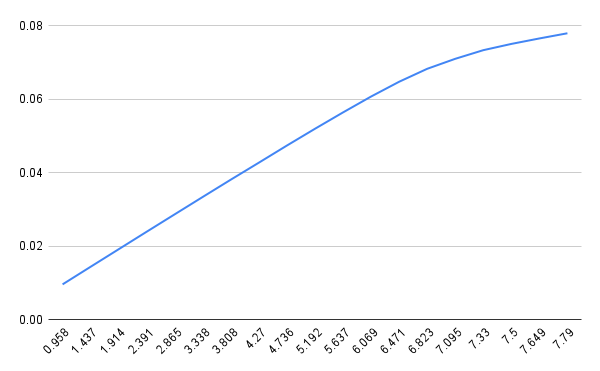
\includegraphics[width=9cm]{chart}}
	\end{figure}
	
		\nchapter{MOSFET Bias Circuit}
	\nsection{Design Objective} In this lab we bias a MOSFET for use in both saturation and triode regions. This allows us to maintain a stable DC operating point.
	\nsection{Circuit Design Outline}
	Using our calculated resistors of $38.2k\Omega$ and $95.3k\Omega$ combined with our given resistance values of $500\Omega$ and $200\Omega$ and connecting them to our NMOS transistor in the configureation shown below we can bias our circuit so that the current across the $500\Omega$ and $200\Omega$ ($I_D$) is 10mA. By inputting a voltage of 15V at the leg of the $500\Omega$ resistor we can achive 10mA across the resistors.
	\begin{figure}[hp!] %140, 
		\centering
		\caption{Bias Circuit}
		\subfloat[Bias Circuit Sim]{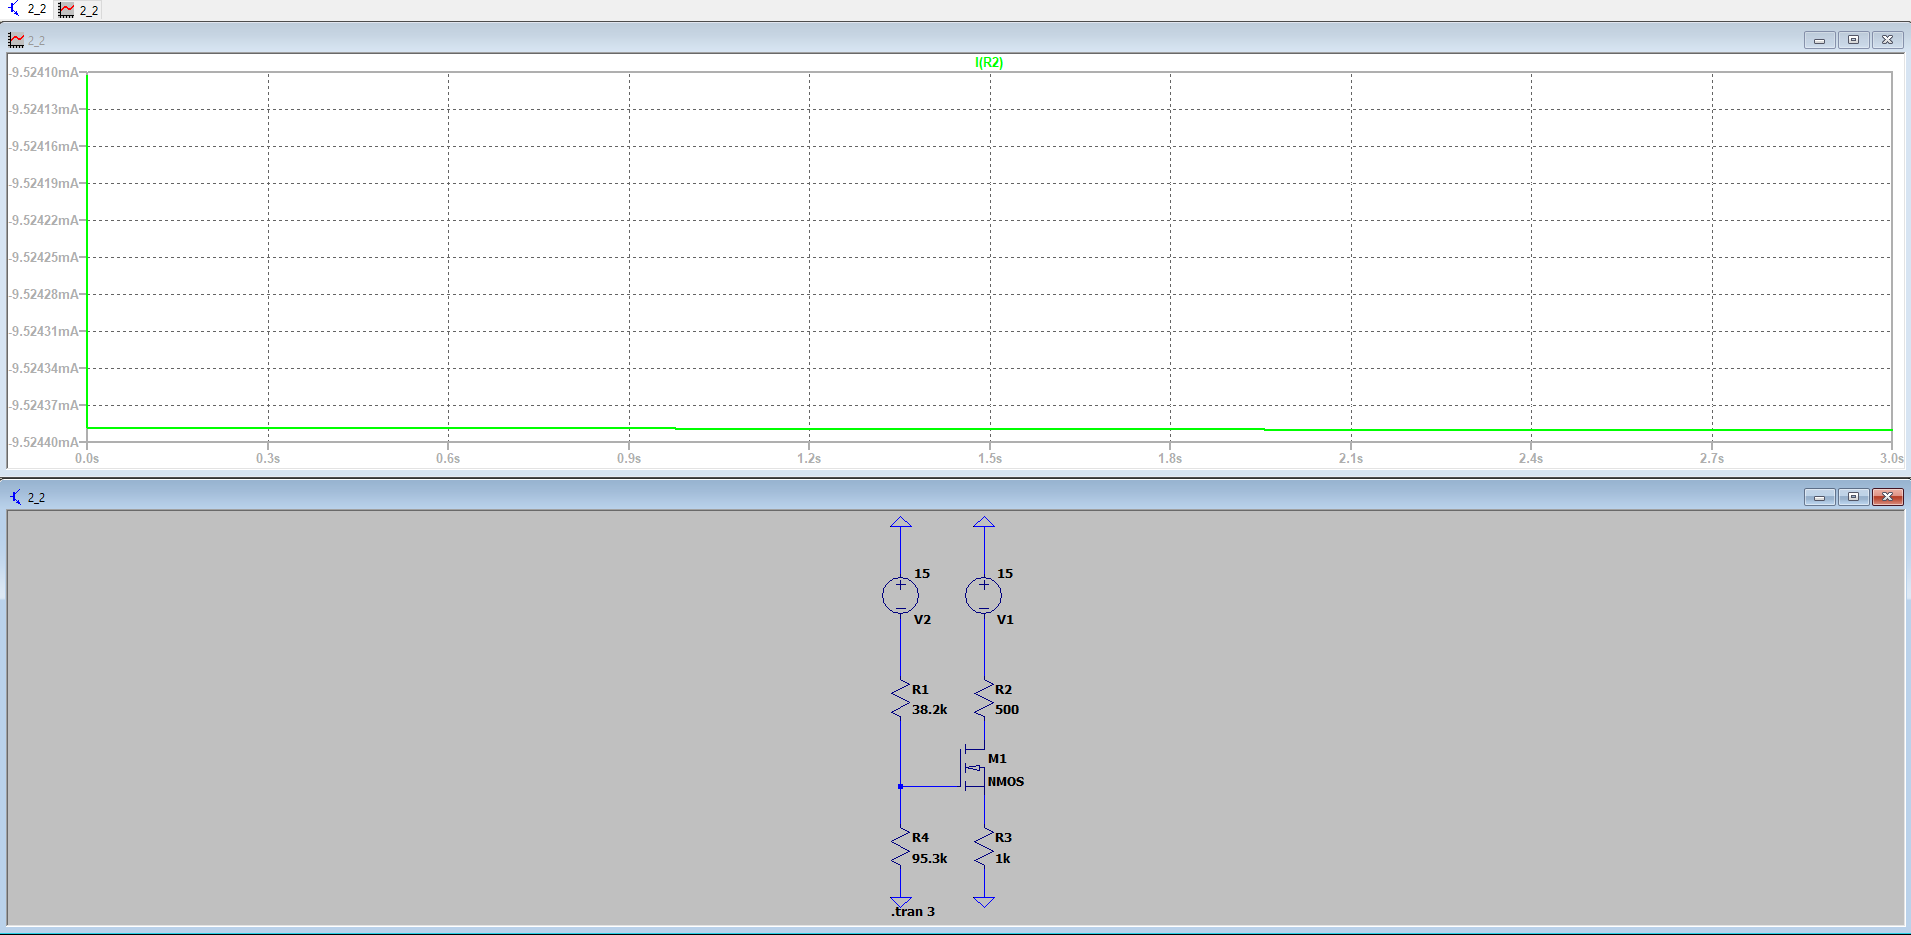
\includegraphics[width=9cm]{SpiceSim}}
	\end{figure}
	\begin{figure}[hp!]
		\ContinuedFloat
		\centering
		\subfloat[\centering Bias Circuit Image]{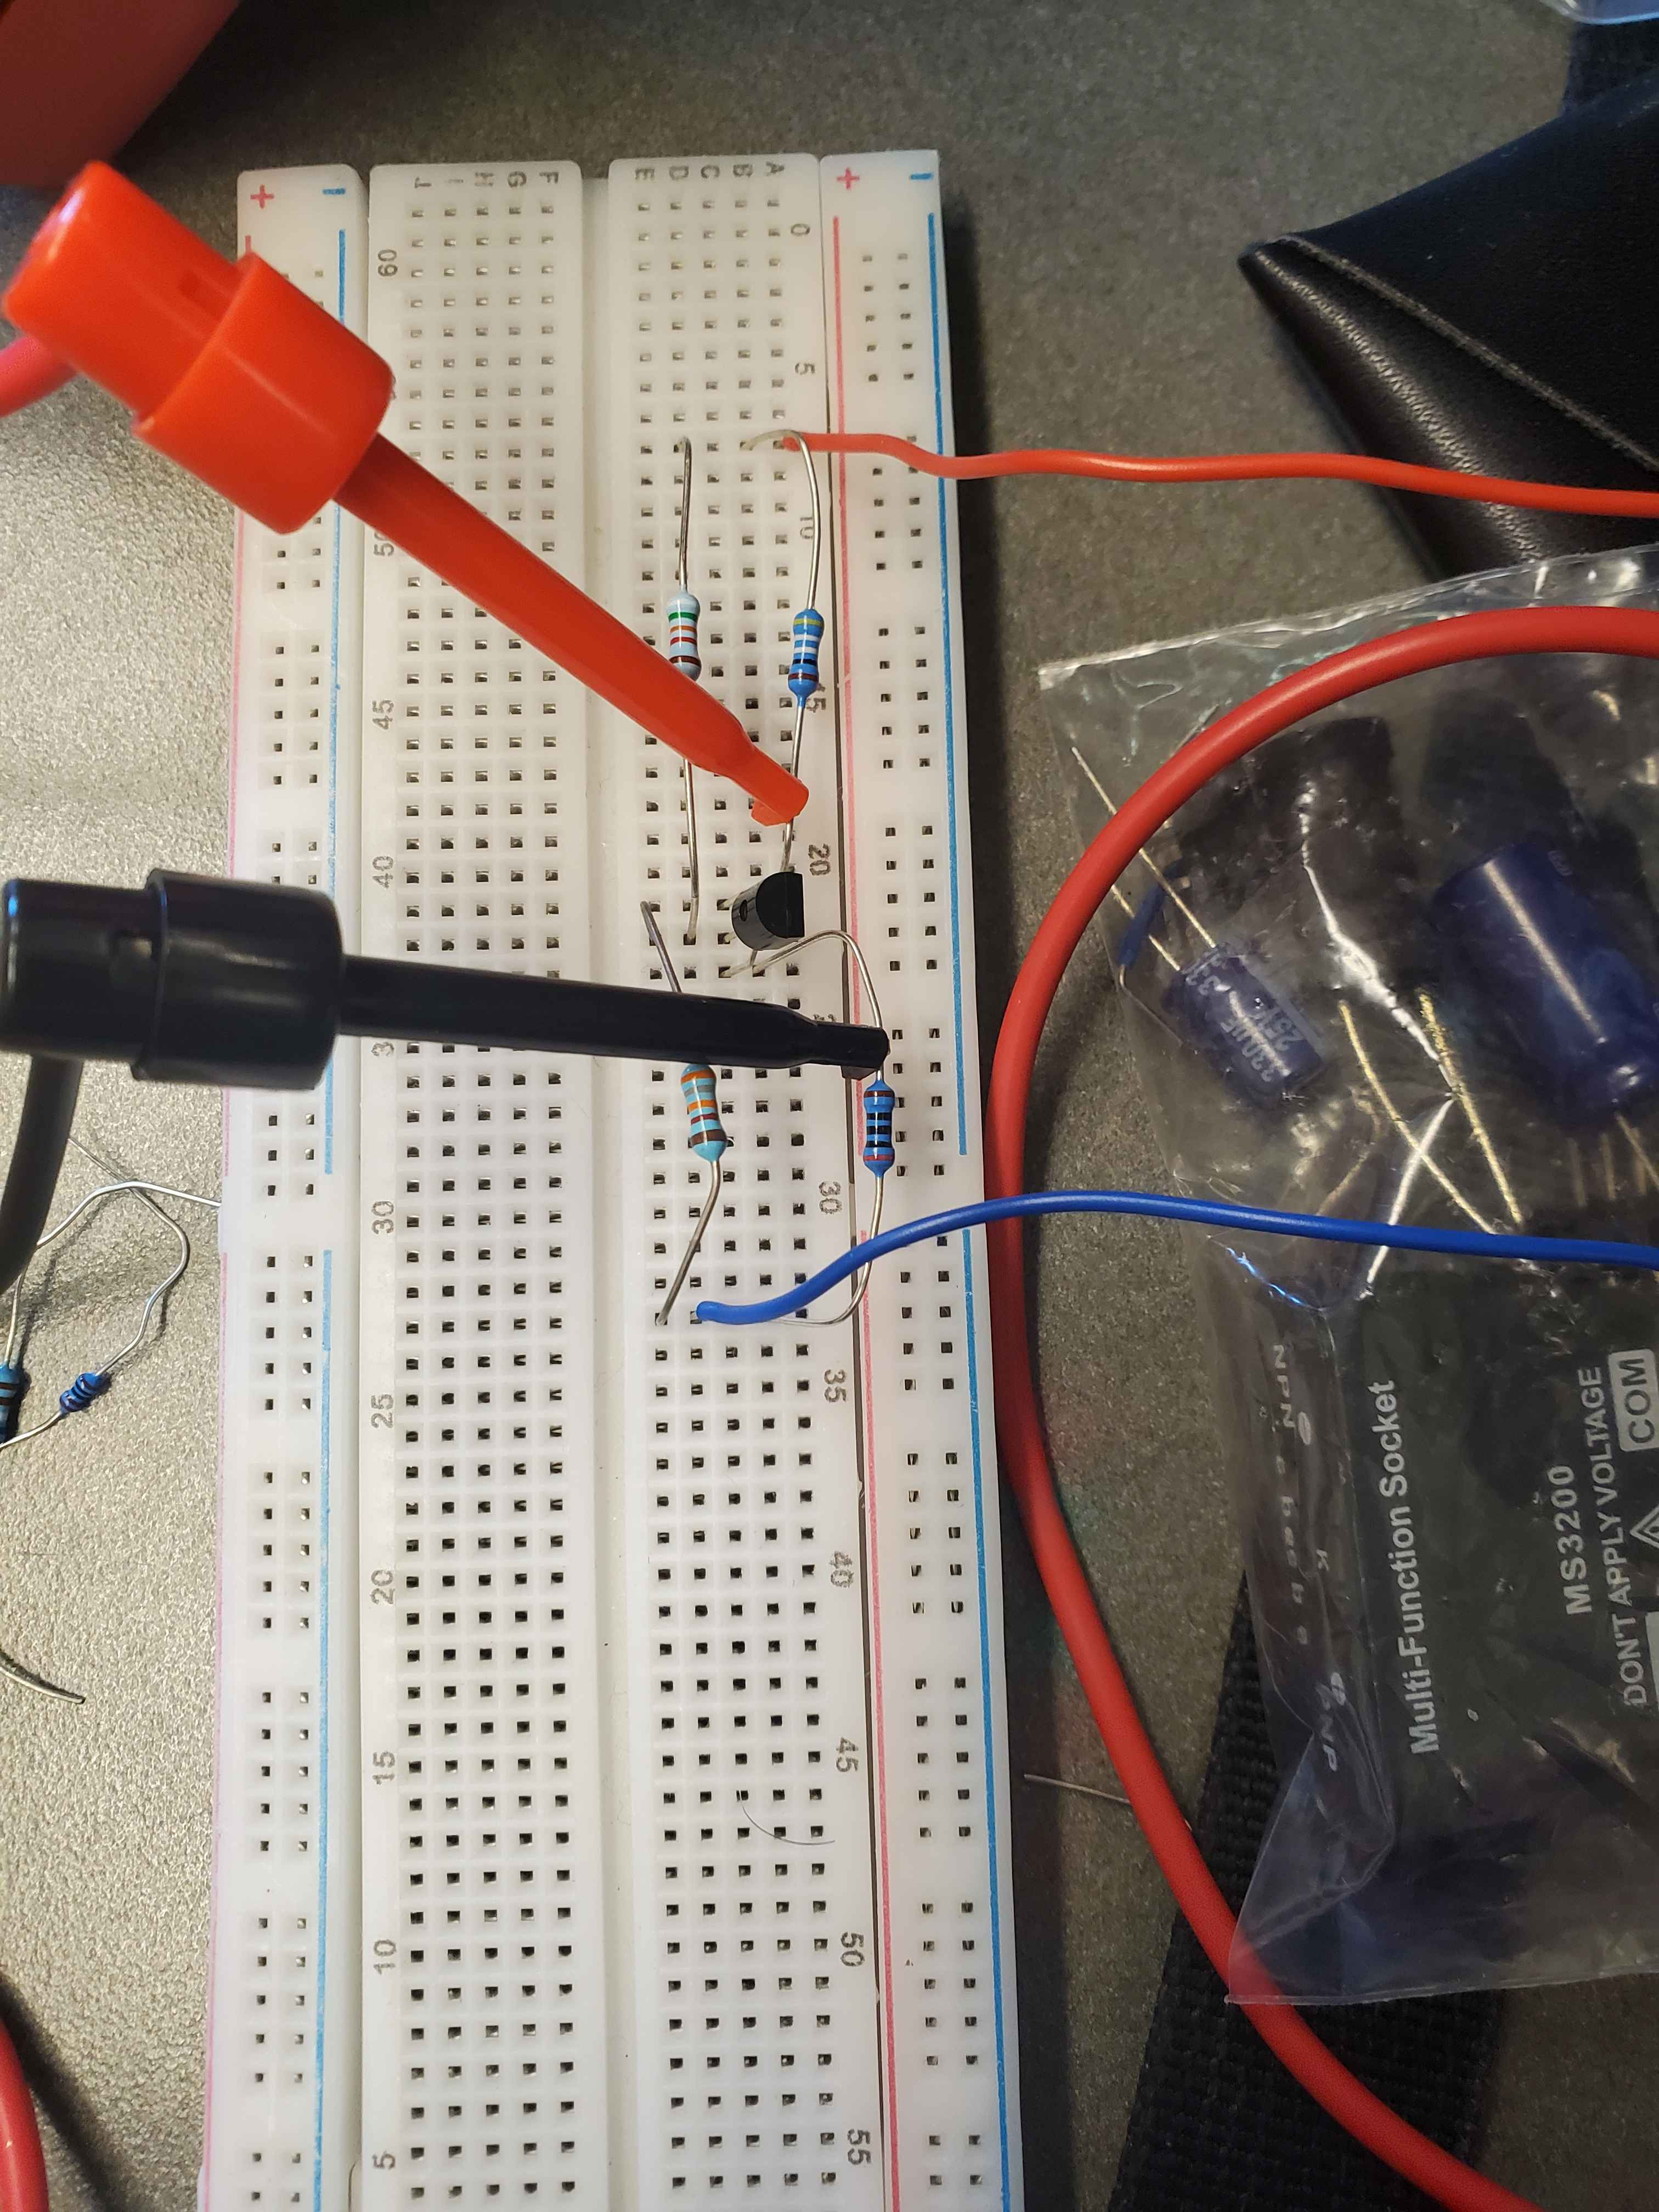
\includegraphics[width=6cm]{CircuitImage}}\hfil
		\subfloat[Bias Circuit Measurement]{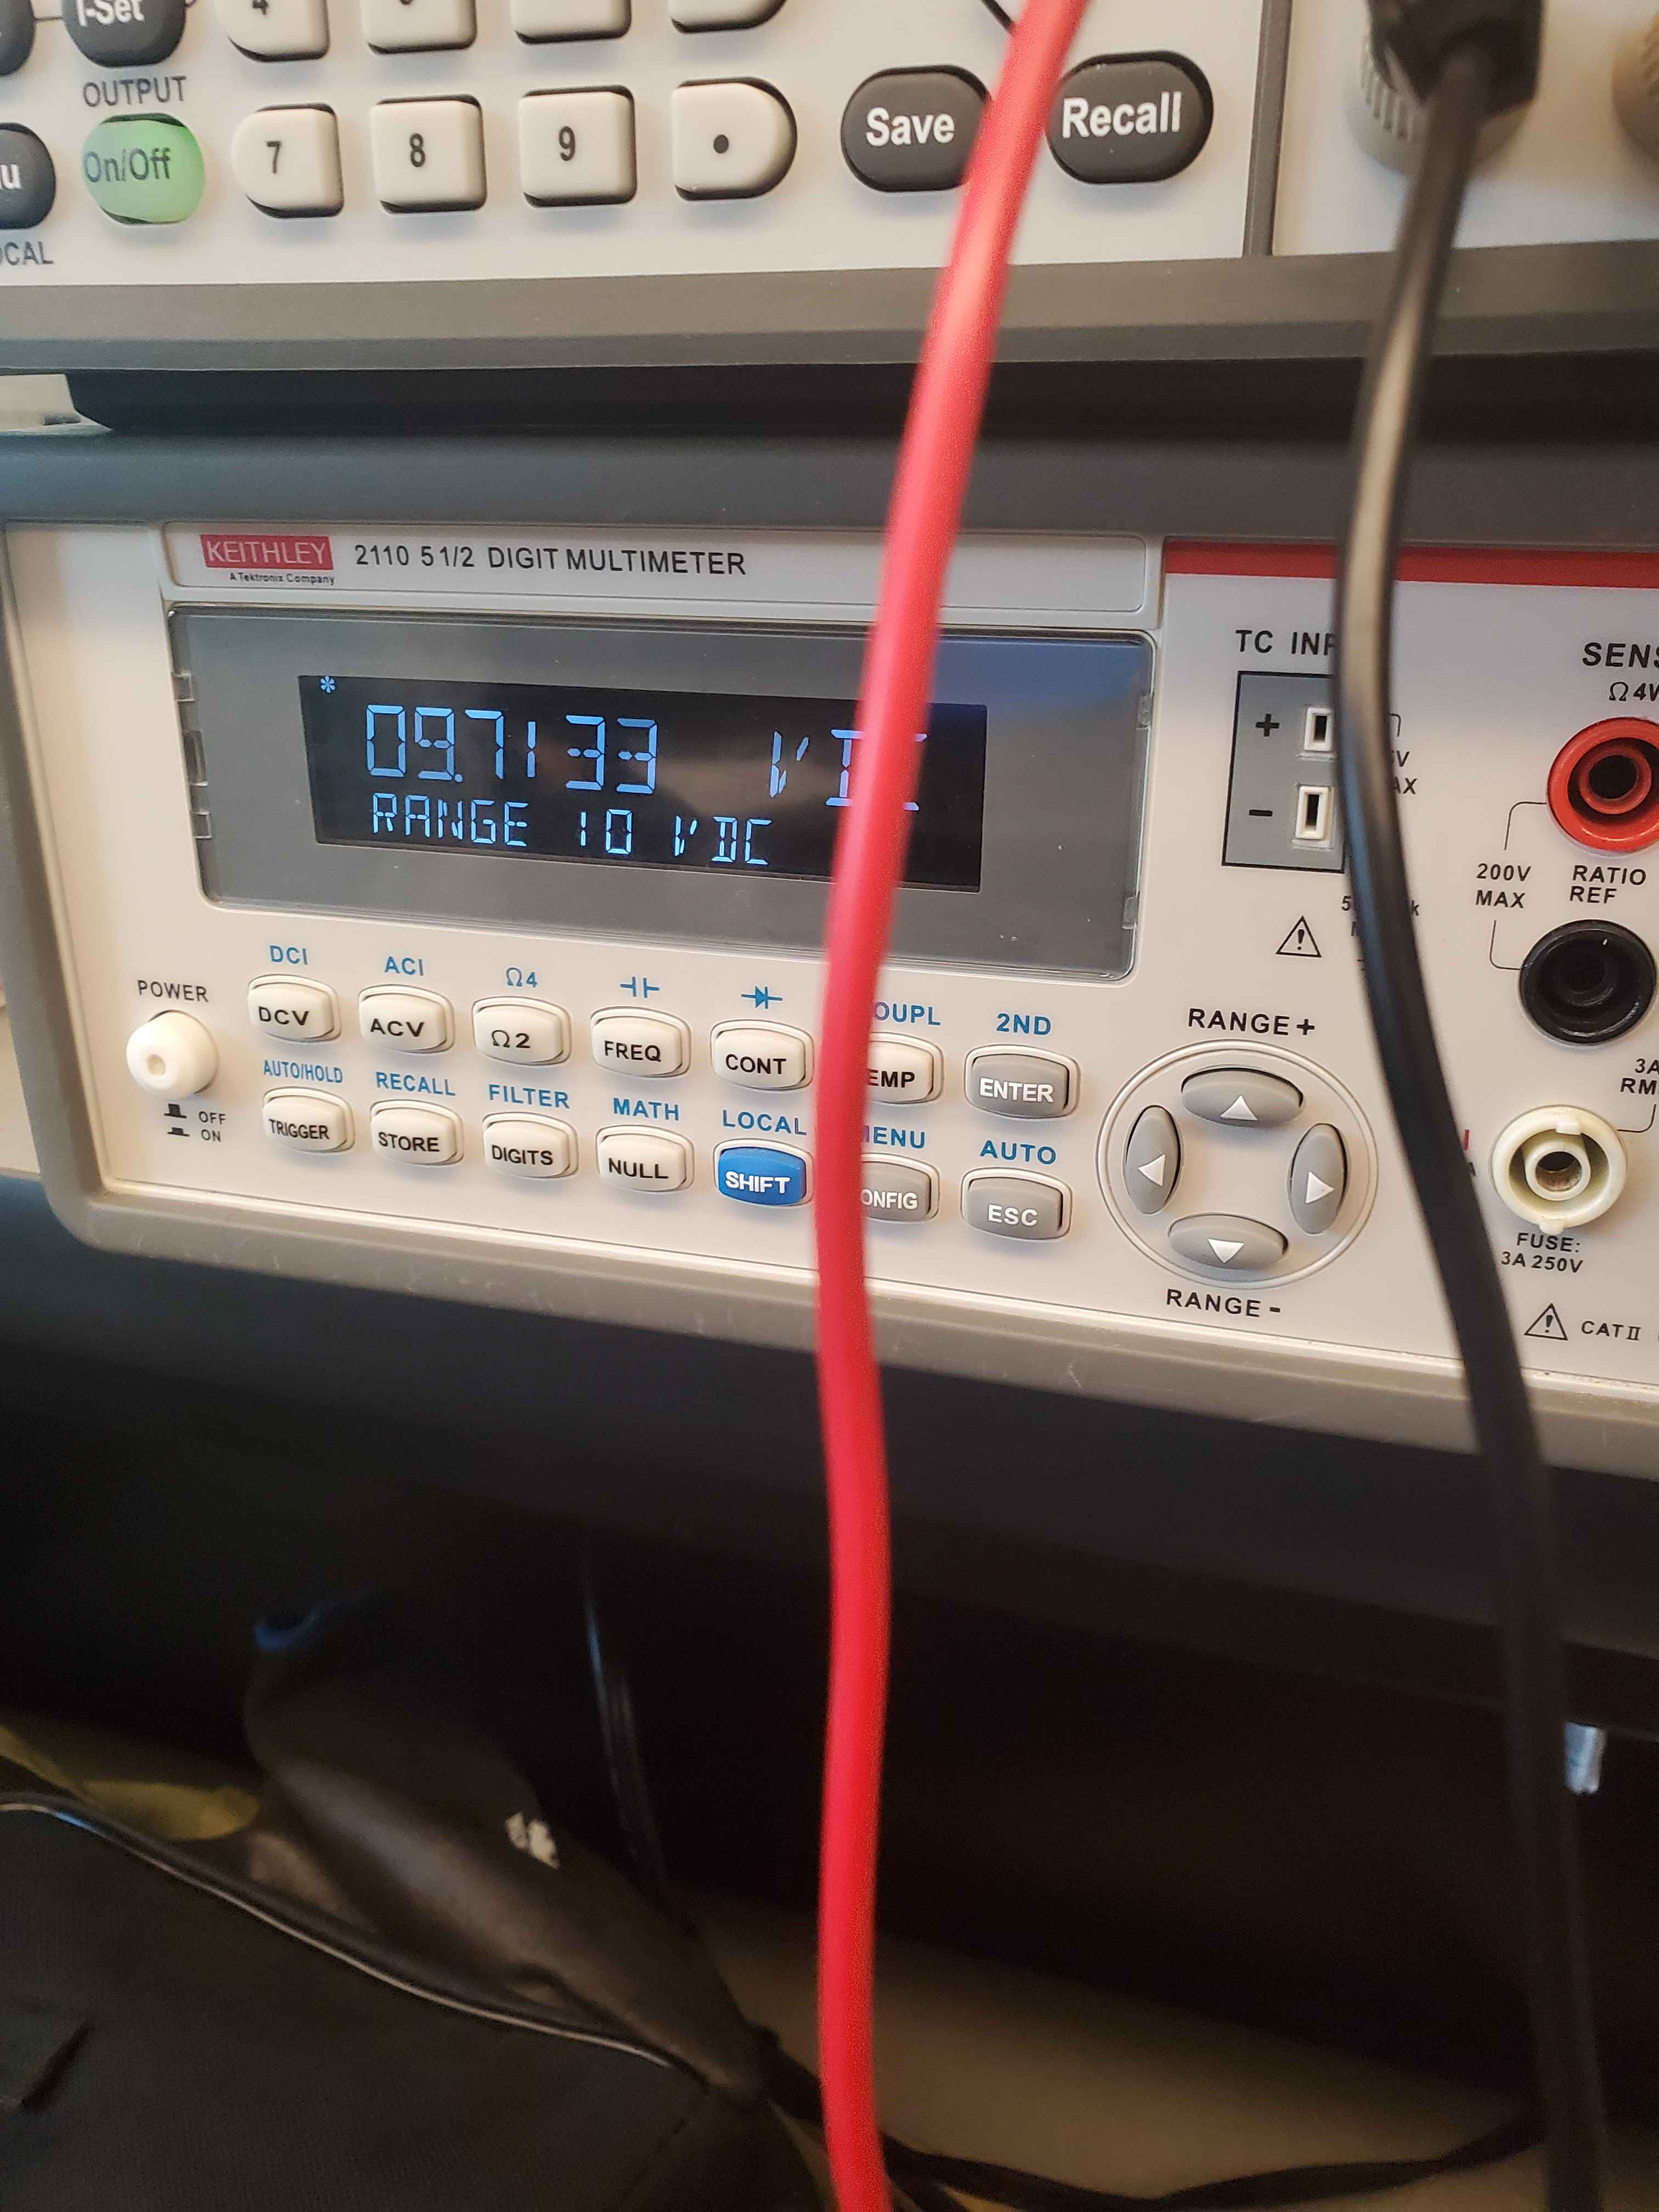
\includegraphics[width=6cm]{VoltageReading}}
	\end{figure}
	\newpage
	\nsection{Measurement and Simulation Results}
	\nsubsection{Analysis}
	\begin{itemize}
		\item \textbf{1. Calculate expected $V_G$, $I_D$ and $V_{DS}$}
		\subitem Using $V_{GS}$ = $V_G$	- $V_S$ and a voltage divider accross the $38.2k\Omega$ and $95.3k\Omega$ resistors we find that $V_G$ = 10.708V.
		\subitem Using the equation $I_D = k_n(V_{GS} - V_T)^2$ we can solve for $I_D$ obtaining $I_D = 10.84mA$ using $k_n = 0.0011$ and $V_T = 1.6$
		\subitem $V_{DS}$ is therefore found using $V_{DS}$ = $V_D$	- $V_S$ where $V_D$ is found using $I_D$, $V_{DD},$ and the $500\Omega$ resistor. This gives us $V_{DS} = 7.411V$
		\item \textbf{2. Compare to simulated results for $V_G$, $I_D$ and $V_{DS}$}
		\subitem The simulated results for $V_G$, $I_D$ and $V_{DS}$ all line up with what we observed during our measurements. The \% difference between the calculated and simulated values are found at a 2\% difference (10.84mA vs 11.04mA).
		\item \textbf{3. Comment on discrepancies}
		\subitem Discrepancies appear from the natural impedance of the NMOS transistor; and the transience of the Gate-Voltage causing a natural and slow rise. As Semiconducting Materials in real life are difficult to keep at a consistent voltage due to them being VERY sensitive and dependent on temperature.
		\subitem 
	\end{itemize}
	
	\nsection{Summary \& Conclusions}
	In this lab, we analysed; characterised; and designed with an NMOSFET transistor for the $I_D$ over both the $V_{GS}$ and $V_{DS}$ region, but also the biasing effects of voltage-dividing over $V_G$
	
	\newpage
	\nchapter{Addendum Pages}
	\begin{figure}[hp!]
		\centering
		\caption{Jason Truong Addendum}
		\subfloat[\centering Lab Design   Calculations]{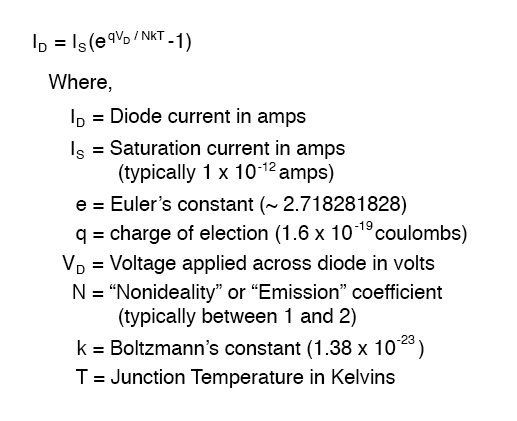
\includegraphics[width=17cm]{Theoretical Calculation of Ideal Diode}}
	\end{figure}
	\newpage
	\nsection{Bibliography}
	\textbf{Cited:}\\
	\begin{itemize}
		\item Lab 1 Manual
		\item Sedra, Adel, and Kenneth Smith. Microelectronic Circuits. S.L., Oxford Univ Press Us, 2019.
	\end{itemize}
	\begin{figure}[!h]
		\subfloat[Keep believing in yourself.]{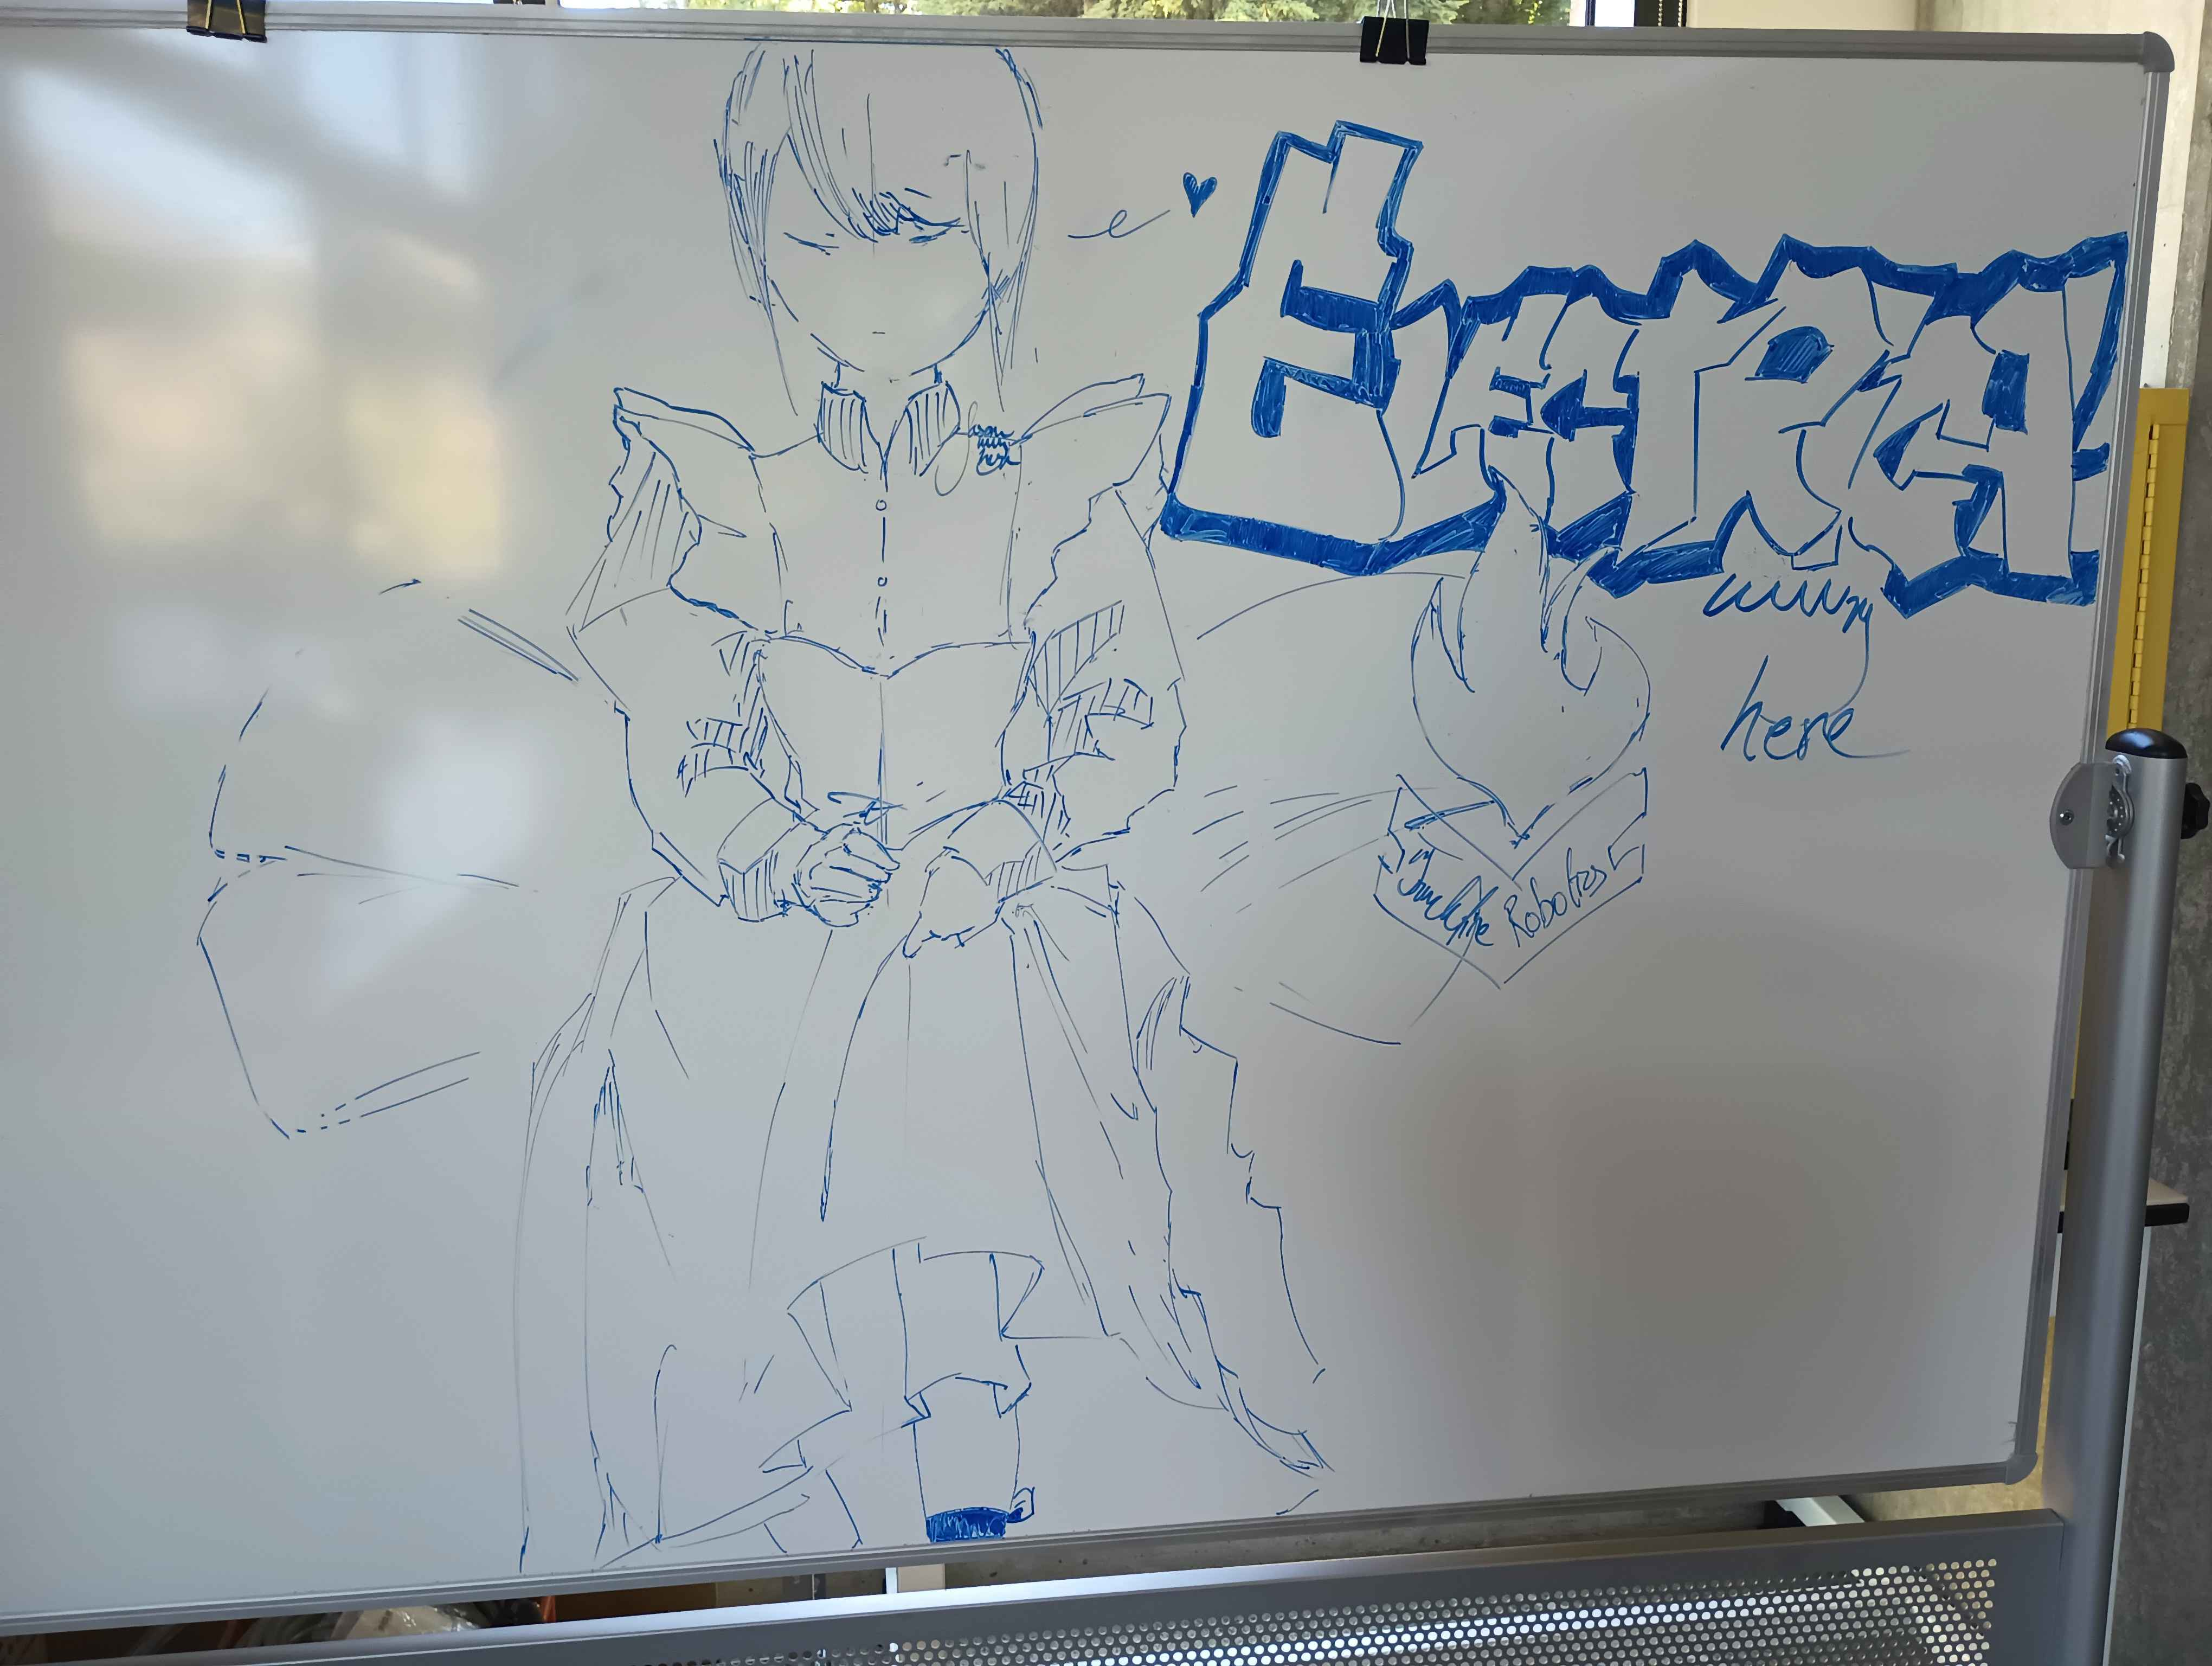
\includegraphics[width=\linewidth]{IMG_20240705_171509323}}
	\end{figure}
\end{document}